\section{Selection Process} 

About the 4 techniques..

\subsection[Triangulation]{Triangulation\footnote{Stefan}} %stefan
\subsubsection*{Summary}
Since our plant has a specified size in which the location of multiple objects has to be performed the method of Triangulation is one promising technic in which research was made. 
Triangulation was already a common principle of measurement in the 18th century and it´s divided between active and passive triangulation. Passive triangulation is a geometrical method based on two measurement stations which positions are known exactly. At these two measurement points angels of the desired point in space are measured to compute the localization in the specified coordinate system (x, y, z) with trigonometrical formulas.
With respect to the two measurement points which were already used in the 18th century nowadays two cameras are installed to perform a geographical method of 3D object-data estimation fig. \ref{Triangulation} \cite{Prinzip3DVideometrie.}.
\begin{figure}[!htbp]
\centering
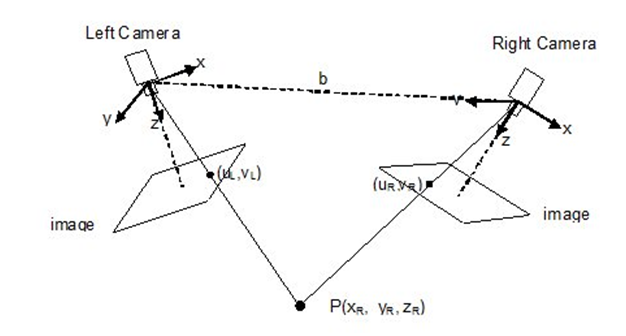
\includegraphics[width = 16cm]{Pictures/Triangulation}
\caption{Passive Triangulation set-up with two cameras}
\label{Triangulation}
\end{figure}\\
To Solve the problem, it is necessary to know the parameters of the left and the right camera visualized in the figure. In theory the triangulation is trivial, since each and every point of the images of the respective cameras maps to a line in 3D space. If a pair of corresponding points, in the case of the pipes less plant it would be an AGV, is found the projection of a point x in 3D space can be computed. 
Active triangulation in comparison to passive triangulation needs one camera and at least one source of structured light (e.g. Laser). As the passive way here the geometrical location and orientation of the camera and light source is space need to be known. Two possible set-ups with either a laser point and a stripe as structured light are shown in fig. \ref{ative_Triangulation} \cite{MultiObjectTriangulation.}.
\begin{figure}[!htbp]
\centering
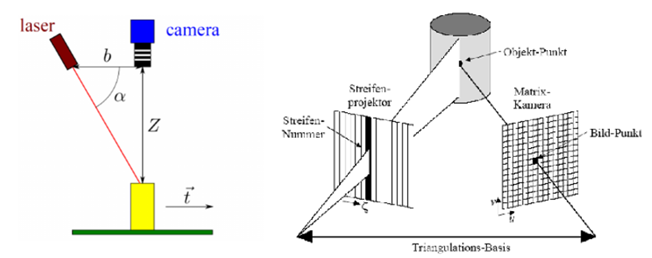
\includegraphics[width = 16cm]{Pictures/acticetriangulation}
\caption{Active Triangulation}
\label{ative_Triangulation}
\end{figure}\\
To solve the active triangulation problem, the structured light has to point on object which location is desired to estimate, in the case of the pipe less plant it would be the AGV. If this point is found on the 2D image of the camera, a triangulation with basic trigonometrical formulas which are using the properties and parameters of the camera and light source can be performed and the position of the AGV is estimated. 
\pagebreak
\subsubsection*{Implementation} 
One possible way to implement a solution for the passive triangulation is to attach 2 high resolution cameras with USB 3.0 for a fast data transmitting on two edges of the plant being not on each others opposite side as shown in fig. \ref{ativeTriangulationimplementation}.\\
\begin{figure}[!htbp]
	\centering
	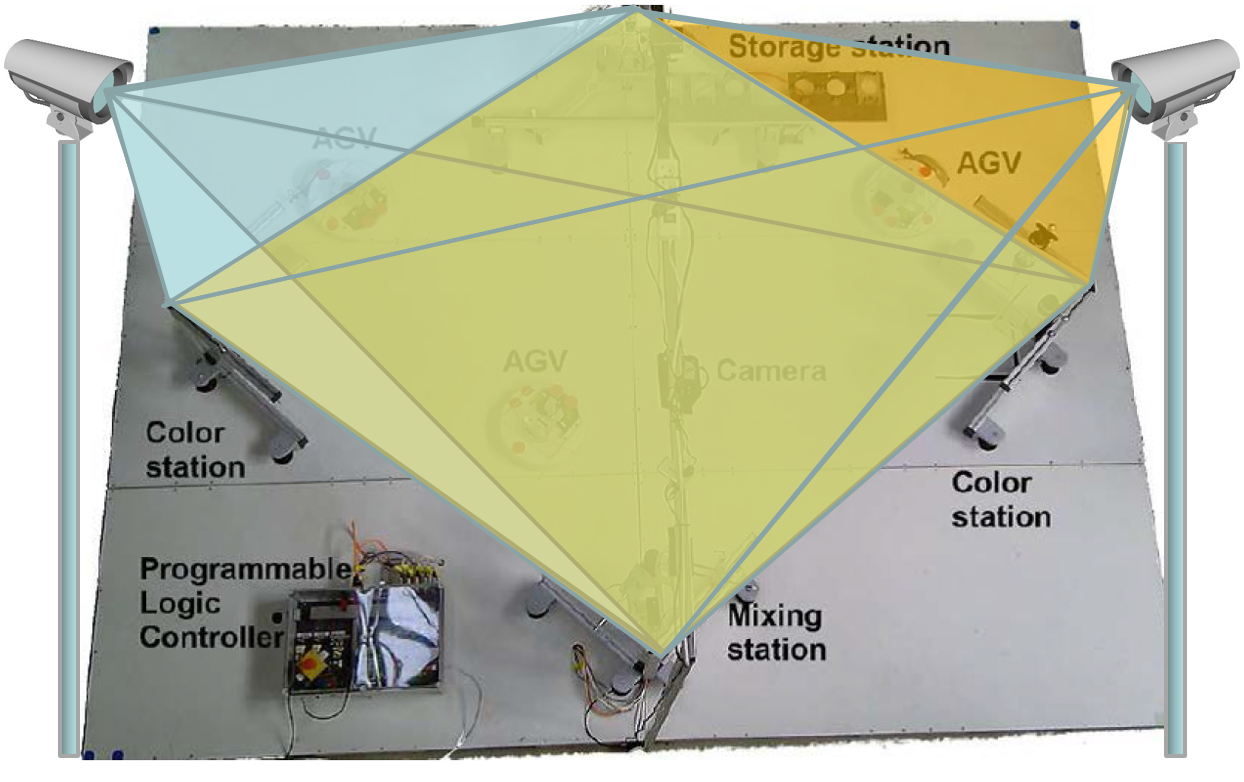
\includegraphics[width = 16cm]{Pictures/triangulationimplementatio}
	\caption{Impmentation of passive triangulation}
	\label{ativeTriangulationimplementation}
\end{figure}\\%
The left and right camera are sequentially taking pictures which are transmitted to the plants computer where the image processing takes place. 
\pagebreak
\subsubsection*{Pro and con}
Based on the made research, two tables with advantages and disadvantages of the two RFID systems are created.
\begin{table}[!htbp]
\centering
\begin{tabular}{|l|l|}
\hline
\multicolumn{2}{|c|}{\textbf{Passive Triangulation}}                                                                                                                  \\ \hline
\multicolumn{1}{|c|}{\textbf{Positive}}                                                                                    & \multicolumn{1}{c|}{\textbf{Negative}}   \\ \hline
Upgrade to USB 3.0 for faster data transmitting possible                                                                   & Light dependent                          \\ \hline
\begin{tabular}[c]{@{}l@{}}Upgrade to a camera with higher resolution to reduce \\ measurement error possible\end{tabular} & New concept of orientation may be needed \\ \hline
No Fish-Eye-Lense problem                                                                                                  & Limited range of observation             \\ \hline
Low cost                                                                                                                   &                                          \\ \hline
\end{tabular}
\caption{Positive and Negative Points of Passive Triangulation}
\label{pro_con_passive_tri}
\end{table}
\begin{table}[!htbp]
\centering
\begin{tabular}{|l|l|}
\hline
\multicolumn{2}{|c|}{\textbf{Active Triangulation}}                                                                                                                     \\ \hline
\multicolumn{1}{|c|}{\textbf{Positive}}                                                                                    & \multicolumn{1}{c|}{\textbf{Negative}}     \\ \hline
Upgrade to USB 3.0 for faster data transmitting possible                                                                   & New unknown laser technology is needed     \\ \hline
\begin{tabular}[c]{@{}l@{}}Upgrade to a camera with higher resolution to reduce \\ measurement error possible\end{tabular} & High costs for several Laser (one per AGV) \\ \hline
Easy detection of laser points on camera image                                                                             & Laser needs to move while AGVs are moving  \\ \hline
                                                                                                                           & Limited range of observation               \\ \hline
                                                                                                                           & Light dependent                            \\ \hline
\end{tabular}
\caption{Positive and Negative Points of Active Triangulation}
\label{pro_con_active_tri}
\end{table}
\pagebreak
\subsection{Pattern Recognition} %medhini
\subsubsection*{Summary} 
\subsubsection*{Implementation}
\subsubsection*{Pro and con}
\pagebreak

\subsection[RFIS]{RFID\footnote{Stephan}} % stephan around 2 pages
\subsubsection*{Summary} 
One of the possible solutions to solve the challenging problem of indoor localization is the use of the Radio-frequency Identification (RFID) technology. The mainly areas of this technology is indeed still supply chains, transport, manufacturing, personnel access, animal tagging, toll collection \textcolor{red}{reference 4}, but has also become popular in localizing objects and persons. Where in the main applications only the identification has to be realized, also the strength of the signals is important to estimate the position of a certain object.\\
The main idea of those systems is that a reader detects a tag and reads its information. The technology can be divided into three main types: passive, semi-passive and active systems. A passive system, like it is been shown in fig. \ref{RFID_Passive}, consists of a reader, which is connected to an antenna and a computer and a passive tag.\\
\begin{figure}[!htbp]
\centering
\begin{minipage}{.5\textwidth}
\centering
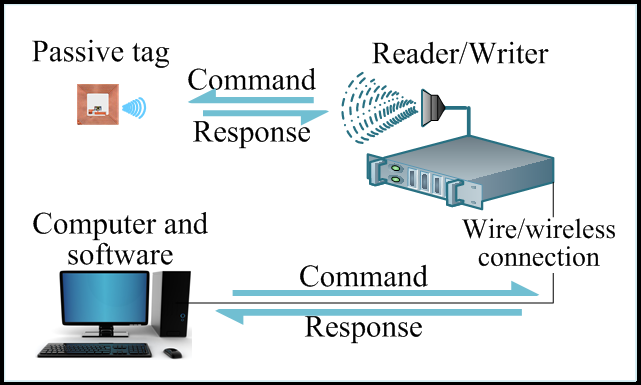
\includegraphics[width = 7cm]{Pictures/RFID_Passive}%
\caption{Passive RFID System}
\label{RFID_Passive}
\end{minipage}%
\begin{minipage}{.5\textwidth}
\centering
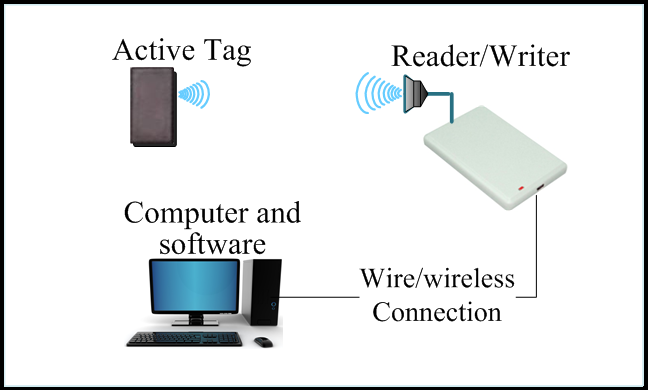
\includegraphics[width = 7cm]{Pictures/RFID_Active}%
\caption{Active RFID System}
\label{RFID_Active}
\end{minipage}
\end{figure}\\
The system is called passive, because the power supply will be realized by the radio signal of the reader. In case where the tag is in the reading range of the reader, the tags gets enough power to send predefined information (for example ID) back. The active system (see fig.\ref{RFID_Active}) in comparison has an active tag which has an own power supply. The semi-passive tag has a battery build in that the the tag has more power to communicate, but is not used to generate radio frequency signals.\\ 
Another classification of RFID systems is the frequency of the radio waves. It can reach from 0.135 MHz (Low Frequency) to 5875 MHz (Super High Frequency). The table \ref{RFID_Systems} gives an overview about the systems related to reading ranges, reading rates and the ability to read near metal or water.\\
\begin{table}[!htbp]
\centering
\begin{tabular}{c}
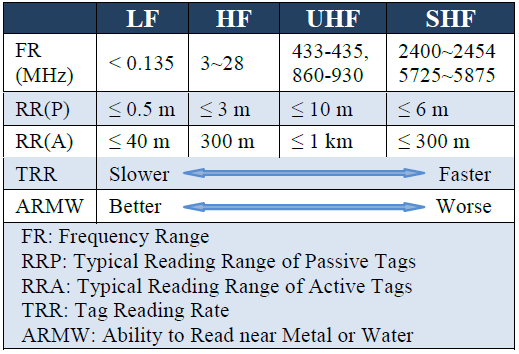
\includegraphics[width = 9cm]{Pictures/RFID_Systems}
\end{tabular}
\caption{Overview RFID systems}
\label{RFID_Systems}
\end{table}\\
It can be seen that the passive systems in general have a smaller reading range then the active systems and has a bigger data rate. But it has also to be take into account, that passive tags a way cheaper then active tags.   
\subsubsection*{Implementation}
There are mainly two different ways to realize a localization system of the AGVs in the pipeless plant. Based on the fact that the plant has a size of 3 by 4 meter, the tracking can be carried out by passive system in which a couple of passive tags on the floor can be used as landmarks. In this case the reader plus the antenna would be placed on the AGV and localize with the help of the detected tags. The other systems consists of three or four reader in each corner of the plant and an active tag on each AGV.
\pagebreak
\subsubsection*{Pro and con}
Based on the made research, two tables with advantages and disadvantages of the two RFID systems are created.\\ 
\begin{table}[!htbp]
\centering
\begin{tabular}{|l|l|}
\hline
\multicolumn{2}{|c|}{\textbf{Active RFID system}}                                                                                                                                                                                \\ \hline
\multicolumn{1}{|c|}{\textbf{Pro}}                                                                                & \multicolumn{1}{c|}{\textbf{Con}}                                                                            \\ \hline
Light independent                                                                                                 & Prototype more expansive (3 reader + avtive tags)                                                            \\ \hline
Space unlimited                                                                                                   & \begin{tabular}[c]{@{}l@{}}Datarate is related to the amount of\\ detected tags a the same time\end{tabular} \\ \hline
\begin{tabular}[c]{@{}l@{}}Localization only has to be realized in\\ a bigger area - medium accuracy\end{tabular} & \begin{tabular}[c]{@{}l@{}}Anticollision need, cause more AGVs are\\ used at the same time\end{tabular}      \\ \hline
\begin{tabular}[c]{@{}l@{}}Wired communication between reader and \\ computer possible\end{tabular}               & \begin{tabular}[c]{@{}l@{}}Signal strength can be influenced by envirnonment\\ (metal or water)\end{tabular} \\ \hline
Simple algorithm (Trilateration)                                                                                  &                                                                                                              \\ \hline
\end{tabular}
\caption{Pro and cons of active RFID system}
\label{my-label}
\end{table}
\begin{table}[!htbp]
\centering
\begin{tabular}{|l|l|}
\hline
\multicolumn{2}{|c|}{\textbf{Passive RFID system}}                                                                                                                                                                                            \\ \hline
\multicolumn{1}{|c|}{\textbf{Pro}}                                                                                             & \multicolumn{1}{c|}{\textbf{Con}}                                                                            \\ \hline
Light independent                                                                                                               & \begin{tabular}[c]{@{}l@{}}Communication between AGV and computer \\ has to be realized\end{tabular}         \\ \hline
Space unlimited                                                                                                                & \begin{tabular}[c]{@{}l@{}}Data rate is related to the amount of\\ detected tags a the same time\end{tabular} \\ \hline
\begin{tabular}[c]{@{}l@{}}Localization only has to be realized between\\ four tags (small area) - high accuracy\end{tabular} & \begin{tabular}[c]{@{}l@{}}Anticollision need, cause more tags are\\ detected at the same time\end{tabular}  \\ \hline
Simple algorithm (Trilateration)                                                                                               &                                                                                                              \\ \hline
Prototype cheap (1 reader + passive tags)                                                                                      &                                                                                                              \\ \hline
\end{tabular}
\caption{Pro and cons passive RFID system}
\label{Pro and Cons of the passive RFID system}
\end{table}
\pagebreak
\subsection{Map-Based Localization} %abdul
\subsubsection*{Summary} 
\subsubsection*{Implementation}
\subsubsection*{Pro and con}
..


